\documentclass{standalone}
\usepackage{tikz}
\usetikzlibrary{arrows}
\usetikzlibrary{decorations.markings}
\begin{document}
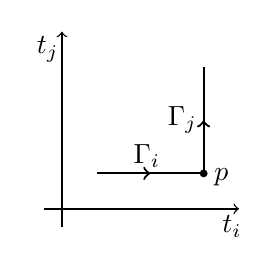
\begin{tikzpicture}[scale=(0.45),arrow/.style={->, >=angle 90},decoration={
    markings,mark=at position 0.5 with {\arrow{>}}}]
    
\draw [->,line width=.5pt] (-.5,0) -- (5,0);
\draw [->,line width=.5pt] (0,-.5) -- (0,5);
\node at (4.8,-.5) {$t_i$};
\node at (-.4,4.5) {$t_j$};

\draw [postaction={decorate},line width=.8pt] (1,1) -- (4,1);
\node at (2.4,1.5) {$\Gamma_i$};
\draw [postaction={decorate},line width=.8pt] (4,1) -- (4,4);
\node at (3.4,2.5) {$\Gamma_j$};

\node [circle, fill=black,inner sep=0, minimum size=1mm] at (4,1) {};
\node at (4.5,.9) {$p$};

%\node at (2.5,.-1.5) {$(+1,+1)$};
%
%\draw (6,-2) -- (6,5.5);
%\begin{scope}[xshift=7.5cm]
%	\draw [->,line width=.5pt] (-.5,0) -- (5,0);
%	\draw [->,line width=.5pt] (0,-.5) -- (0,5);
%	\node at (4.8,-.5) {$t_i$};
%	\node at (-.4,4.5) {$t_j$};
%	
%	\draw [postaction={decorate},line width=.8pt] (1,4) -- (4,4);
%	\node at (2.4,3.4) {$S_i$};
%	\draw [postaction={decorate},line width=.8pt] (4,4) -- (4,1);
%	\node at (3.4,2.5) {$S_j$};
%	
%	\node [circle, fill=black,inner sep=0, minimum size=1mm] at (4,4) {};
%	\node at (4.4,3.9) {$p$};
%	\node at (2.5,.-1.5) {$(+1,-1)$};
%\end{scope}
%
%\draw (13.5,-2) -- (13.5,5.5);
%\begin{scope}[xshift=15cm]
%	\draw [->,line width=.5pt] (-.5,0) -- (5,0);
%	\draw [->,line width=.5pt] (0,-.5) -- (0,5);
%	\node at (4.8,-.5) {$t_i$};
%	\node at (-.4,4.5) {$t_j$};
%	
%	\draw [postaction={decorate},line width=.8pt] (4,1) -- (1,1);
%	\node at (2.5,1.6) {$S_i$};
%	\draw [postaction={decorate},line width=.8pt] (1,1) -- (1,4);
%	\node at (1.6,2.5) {$S_j$};
%	
%	\node [circle, fill=black,inner sep=0, minimum size=1mm] at (1,1) {};
%	\node at (.6,.9) {$p$};
%	\node at (2.5,.-1.5) {$(-1,+1)$};
%\end{scope}
%
%\draw (21,-2) -- (21,5.5);
%\begin{scope}[xshift=22.5cm]
%	\draw [->,line width=.5pt] (-.5,0) -- (5,0);
%	\draw [->,line width=.5pt] (0,-.5) -- (0,5);
%	\node at (4.8,-.5) {$t_i$};
%	\node at (-.4,4.5) {$t_j$};
%	
%	\draw [postaction={decorate},line width=.8pt] (4,4) -- (1,4);
%	\node at (2.6,3.4) {$S_i$};
%	\draw [postaction={decorate},line width=.8pt] (1,4) -- (1,1);
%	\node at (1.6,2.5) {$S_j$};
%	
%	\node [circle, fill=black,inner sep=0, minimum size=1mm] at (1,4) {};
%	\node at (.6,3.9) {$p$};
%	\node at (2.5,.-1.5) {$(-1,-1)$};
%\end{scope}
\end{tikzpicture}
\end{document}